\chapter{Conception}
\label{conception}
%note en bas de page

\section{Patron de conception}

%Contenu de la note précédemment marquée avec \footnotemark


Singleton : Utilisé pour notre Logger, un unique objet est instancié lors du premier appel et ce pendant toute la durée de vie du programme.\\
\begin{center}
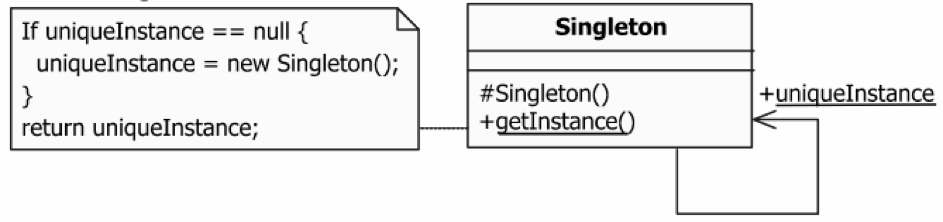
\includegraphics[width=0.60\textwidth]{./assets/singleton.png}~\\
\end{center}


Prototype : Utilisé pour la quasi-totalité des beans Spring. Permets d'instancier plusieurs instances d'objets selon une unique spécification. Très utile pour générer les decks.\\
%retour à la ligne (alinea)
\begin{center}
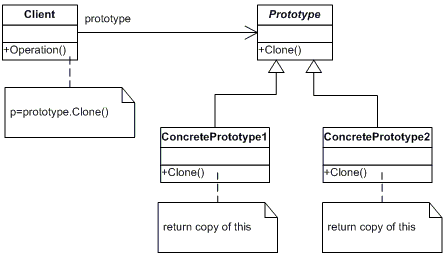
\includegraphics[width=0.60\textwidth]{./assets/prototype.png}~\\
\end{center}
%\includegraphics{./assets/Prototype.png}


Strategy : utilisé pour les stratégies de nos robots. Permets d'encapsuler plusieurs stratégies afin d'avoir une stratégie mère se chargeant de produire le résultat espéré selon une action défini.\\
%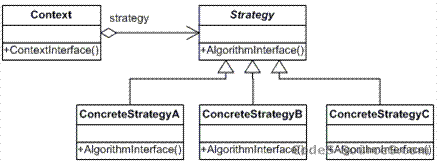
\includegraphics{./assets/strategie.png}
\begin{center}
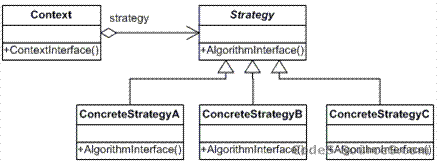
\includegraphics[width=0.60\textwidth]{./assets/strategie.png}
\end{center}
%\newpage
